\documentclass[12pt,a4paper]{article}
\usepackage[latin1]{inputenc}
\usepackage{graphicx}
\usepackage{amsmath}
\usepackage{verbatim,natbib}

\begin{document}

\section*{Exercise}
Consider the following dataset \citep{RoystonSauerbrei2008}:

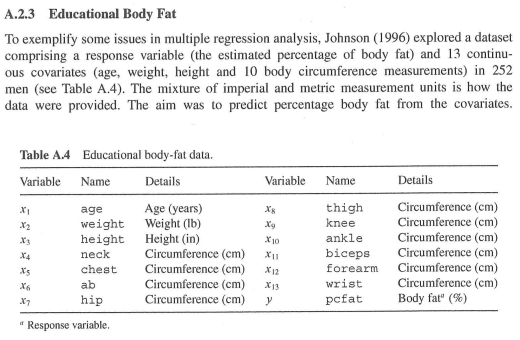
\includegraphics{EBF_description}

\noindent Download the data by using the code in the course web-page (link: Exercises) and perform model selection with:
\begin{itemize}
\item backward elimination;
\item forward selection;
\item stepwise selection;
\item stepback selection;
\item best subset selection
\end{itemize}
Report the regression coefficient estimates (with the corresponding standard errors) and comment the results.

\bibliographystyle{../../../../../support/biometrika}
\bibliography{../../../../../support/biblio}

\end{document}
